\documentclass{article} 
\usepackage{amsmath} 
\usepackage{amssymb} 
\usepackage{amsthm} 
\usepackage[margin=0.2in]{geometry} 
\usepackage{hyperref} 
\usepackage{physics} 
\usepackage{tikz} 
\usepackage{mathtools}
\usepackage{graphicx}\graphicspath{{./images/}}
\mathtoolsset{showonlyrefs} 
\theoremstyle{definition} 
\newtheorem{theorem}{Theorem}[section] 
\newtheorem{corollary}{Corollary}[theorem] 
\newtheorem{lemma}[theorem]{Lemma} 
\newtheorem{definition}{Definition}[section] 

\author{Connor Duncan}
\date{\today}

\title{notes-11-04-2019}
\begin{document}
\abstract{A single document copy of these notes, as well as a mirror of every note, can be found at \url{connorduncan.xyz/notes}}
\subsection{Validity Criterion} This was an aside on the date 11-4-19. We ended up getting a sinc function from the last time. I made an error, last time. WE should actually have \begin{equation} F(t,\omega)=\frac{2\sin[2](\omega_{fi}t/2)}{\omega_{fi}^2t} \end{equation} where in the limit of very large times, $F(t,\omega)\rightarrow\pi\delta(\omega)$. From this\footnote{todo: wtf}, we can get the maximum probability \begin{equation} P_{fi}^{\mathrm{max}}=\frac{2|\bra{f}H_1\ket{i}|^2}{E_f^{(0)}-E_{i}^{(0)}} \end{equation} The validity criterion here is the same roughly as it was previously, where the energy difference should be small. Also, resonant transitions are going to give a really weird case that we need to be extra mindful of. Even if one transition is resonant, it breaks validity of perturbation theory, the true criterion is \begin{equation} \sum_{f}^{}P_{fi}^\mathrm{max}=\sum_{f}^{}\frac{2|\bra{f}H_1\ket{i}|^2}{E_{f}^{(0)}-E_{i}^{(0)}}\ll 1 \end{equation} We're going to move on, we want to take \begin{itemize} \item Static Perturbations $\rightarrow$ Oscillatory Perturbation \item Transition into a Continuum of Levels \end{itemize} We're going to discuss this through the lense of \textbf{Fermi's Golden Rule}. \subsection{Periodic Perturbations} Consider \begin{equation} H_1(t)=\Theta(t)\left[\hat Ve^{-i\omega t}+\hat V^\dag e^{i\omega t}\right] \end{equation} As an example of ramping up a perturbation suddenly. Or, \begin{equation} \bar H_1(t)=e^{\varepsilon t}\left[\hat Ve^{-i\omega t}+\hat V^\dag e^{i\omega t}\right] \end{equation} here $t<0,\varepsilon\ll\frac{2\pi}{t}$ as an example of ramping up slowly. \subsubsection{Sudden Step Into Periodicity} We can just use the first order formalism to get \begin{equation} d_f^{(1)}(t)=-\frac{i}{\hbar}\bra{f}\hbar V\ket{i}\int_{0}^{t}e^{i(\omega_{fi}-\omega)t'}dt' -\frac{i}{\hbar}\bra{f}\hat V^\dag\ket{i}\int_{0}^{t}e^{i(\omega_{fi}+\omega)t'}dt' \end{equation} if we let $V_{fi}=\bra{f}\hat V\ket{i}$, we have \begin{equation} d_f^{(1)}(t)=V_{fi}\frac{1-\exp(i(\omega_{fi}-\omega)t)}{\hbar(\omega_{fi}-\omega)} +V_{fi}^\dag\frac{1-\exp(i(\omega_{fi}+\omega)t)}{\hbar(\omega_{fi}+\omega)} \end{equation} which gives \begin{equation} P_{fi}= \left| V_{fi}\frac{1-\exp(i(\omega_{fi}-\omega)t)}{\hbar(\omega_{fi}-\omega)} +V_{fi}^\dag\frac{1-\exp(i(\omega_{fi}+\omega)t)}{\hbar(\omega_{fi}+\omega)} \right|^2 \end{equation} We have really strong resonances at $\omega=\omega_{fi}$, and decay over time otherwise. This gives us that it's a reasonable approximation to use \begin{equation} P_{fi}=\left\{\begin{matrix*}[l] \frac{2}{\hbar^2}(V_{fi})^2F(t,\omega_{fi}-\omega)t & \omega_{fi}\approx\omega\\ \frac{2}{\hbar^2}(V_{fi}^\dag)^2F(t,\omega_{fi}+\omega)t & \omega_{fi}\approx-\omega \end{matrix*}\right. \substack{\longmapsto\\t\rightarrow\infty} \left\{\begin{matrix*}[l] \pi\delta(\omega_{fi}-\omega) & \omega_{fi}\approx\omega\\ \pi\delta(\omega_{fi}+\omega) & \omega_{fi}\approx-\omega \end{matrix*}\right. \end{equation} \subsubsection{Slowly Ramped Perturbation} Let's consider as an example, the case where we are nearly resonant with the first term of our perturbation $\bar H$. \begin{equation} V(t)=\hat Ve^{\varepsilon t}e^{-i\omega t} \end{equation} Then we have \begin{equation} d_f^{(1)}(t)=-\frac{i}{\hbar}\int_{-\infty}^{t}\hat V_{fi}e^{i(\omega_{fi}-\omega-i\varepsilon)t'}dt' =-\frac{1}{\hbar}\frac{e^{i(\omega_{fi}-\omega-i\varepsilon)t}}{\omega_{fi}-\omega-i\varepsilon} \end{equation} If we consider the probability, we're going to get \begin{equation} P_{fi}(t)=\frac{1}{\hbar^2}\frac{e^{2\varepsilon t}}{(\omega_{fi}-\omega)^2+\varepsilon^2}|V_{fi}|^2 \end{equation} we can ask what is the rate of transitions we make at long times, \begin{equation} W_{fi}=\pdv{P_{fi}}{t}=\frac{2}{\hbar^2}\frac{\varepsilon}{(\omega_{fi}-\omega)^2+\varepsilon^2}|V_{fi}|^2 \end{equation} this is a a Lorenztian! We have some peaked function \begin{center} 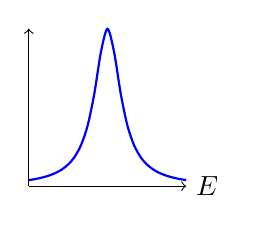
\begin{tikzpicture}[scale=2] \draw[->] (0,0)--(1,0) node[anchor=west]{$E$}; \draw[->] (0,0)--(0,1); \draw[blue,thick] plot[domain=0:1,variable=\x,smooth] ({\x},{.01/((\x-0.5)^2+0.01)}); \end{tikzpicture} \end{center}
\end{document}
